\documentclass[a4paper, 12pt]{article}

\usepackage[portuges]{babel}
\usepackage[utf8]{inputenc}
\usepackage{amsmath}
\usepackage{indentfirst}
\usepackage{graphicx}
\usepackage{multicol,lipsum}
\usepackage{cite}
\usepackage{hyperref}
\usepackage{float}

\begin{document}
%\maketitle

\begin{titlepage}
	\begin{center}
	
	%\begin{figure}[!ht]
	%\centering
	%\includegraphics[width=2cm]{c:/ufba.jpg}
	%\end{figure}

		\Huge{Universidade Federal de São Paulo}\\
		\large{Instituto de Ciência e Tecnologia}\\ 
		\large{Projeto e Análise de Algoritmos}\\ 
		\vspace{15pt}
        \vspace{95pt}
        \textbf{\LARGE{Problema do Caixeiro Viajante}}\\
		%\title{{\large{Título}}}
		\vspace{3,5cm}
	\end{center}
	
	\begin{flushleft}
		\begin{tabbing}
			Alunos: André Vitor Leiniö \\
					\hspace{3.5em}	Davi Melo Morales \\
                   	\hspace{3.5em}	Lucas Santana Lellis
	\end{tabbing}
 \end{flushleft}
	\vspace{1cm}
	
	\begin{center}
		\vspace{\fill}
			 Dezembro\\
		 2015
			\end{center}
\end{titlepage}

% % % % % % % % % % % % % % % % % % % % % % % % % % %
\section{Introdução}
O problema do caixeiro viajante consiste em um problema NP-Completo de otimização combinacional\cite{cormen2009introduction}, que possui grande importância em pesquisa operacional e em ciência da computação teórica. Seu enunciado é o seguinte:
\begin{quote}
``Dada uma lista de cidades e as distâncias entre elas, qual seria a menor rota possível a qual o caixeiro viajante visitasse cada uma delas exatamente uma vez e ao final retornasse à cidade de origem?''
\end{quote}
Sua primeira formulação foi feita em 1930 e hoje é um dos problemas mais estudados na área de otimização, sendo utilizado como \textit{benchmark} para uma série de métodos. Suas aplicações práticas podem abranger áreas como planejamento e logística.

Há diversas possíveis soluções para o problema, tanto de maneira exata - tais como força bruta e \textit{backtracking} - quanto de maneira aproximada, por meio de heurísticas, como o \textit{Simulated Annealing}.

\newpage
\section{Objetivos}

Implementar soluções para o problema do caixeiro viajante e realizar comparações entre a de forma aproximada e a de forma exata, levando em consideração os tempos de execução e a qualidade das soluções aproximadas.

\newpage
\section{Métodos}

Para tal, foram feitas três abordagens para a resolução do problema: a solução por força bruta, por backtracking e pela heurística \textit{Simulated Annealing}.
Para os testes dos algoritimos utilizou-se uma máquina com as especificações descritas na Tabela \ref{tab:cpu}, com as instâncias listadas na Tabela \ref{tab:input}.

\begin{table}[h]

\label{tab:cpu}
\centering
\begin{tabular}{| l |  l |}
 \hline
 CPU & Intel i7 990X \\
 \hline
 Cores & 6\\
 \hline
 Threads & 12\\
 \hline
 Clock & 3.47 GHz\\
 \hline
 Cache& 12 MB \\
 \hline
 RAM & 20 GB \\
 \hline
 SO & Ubuntu 14.04 \\
 \hline
\end{tabular}
\caption{Especificações da Máquina}
\end{table}

\begin{table}[h]

\label{tab:input}
\centering
\begin{tabular}{| l |  l | l | }
 \hline
 \textbf{Nome} & \textbf{Tamanho} & \textbf{Sol. Exata}\\\hline
 Berlim52      & 52               & 7,542               \\\hline
 Pr76          & 76               & 108,159             \\\hline
 Ch150         & 150              & 6,528               \\\hline
\end{tabular}
\caption{Instâncias utilizadas\protect\footnotemark}
\end{table}
\footnotetext{Instâncias e soluções exatas obtidas no endereço \url{http://comopt.ifi.uni-heidelberg.de/software/TSPLIB95/}}
Testes foram feitos utulizando o algoritimo \textit{Simulated Annealing} variando o parametro $\alpha$
entre o valores 0.85, 0.90 e 0.99 e executando o algoritimo duas vezes para cada entrada e anotado o tempo de execução e o resultado.

Testou-se também uma instância de tamanho menor a fim de comparar os tempos de resolução dos algoritmos, assim como a qualidade das soluções obtidas; essa instância apresenta os 13 primeiros valores de Berlim52 e foi chamada de \textit{littleboy}. A Tabela \ref{tab:cpu2} apresenta as especificações da máquina usada para tais testes.

\begin{table}[H]

\label{tab:cpu2}
\centering
\begin{tabular}{| l |  l |}
 \hline
 CPU & Intel® Core™2 Duo CPU E7400 \\
 \hline
 Cores & 2\\
 \hline
 Threads & 2\\
 \hline
 Clock & 2.80 GHz\\
 %\hline
 %Cache& 12 MB \\
 \hline
 RAM & 4 GB \\
 \hline
 SO & Fedora 22 \\
 \hline
\end{tabular}
\caption{Especificações da Máquina 2}
\end{table}


\subsection{Considerações}

A entrada do problema consiste em um arquivo que possui um número sequencial de cidades em que cada linha apresenta uma identificação e as coordenadas nos eixos \textit{x} e \textit{y} de cada cidade.

A representação do problema se deu através de um vetor, no qual as cidades foram identificadas através de uma \textit{id} própria, representada pela Figura \ref{fig:arr}.

\begin{figure}[!ht]
	\centering
		\resizebox{9.5cm}{!}{
		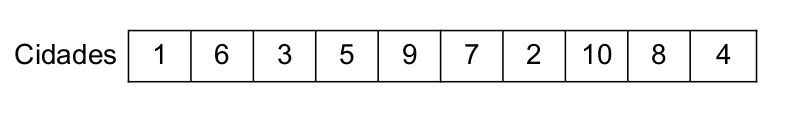
\includegraphics{arrayExample.png}}
	\caption{Exemplo de representação do problema.}
	\label{fig:arr}
\end{figure}

Um pré-processamento é realizado de modo que calculam-se as distâncias euclideanas entre todas as cidades e estes resultados são armazenados em uma tabela para consulta.

\subsection{Força Bruta}

A abordagem por força bruta considera todas as possíveis permutações entre as cidades, calculando a cada iteração o valor da rota presente; comparam-se então os valores para que se encontre o melhor (menor).

Levando-se em conta que nesta implementação é necessário considerar cada permutação entre as \textit{n} cidades de entrada, serão feitas comparações entre as \textit{n!} possíveis soluções e para cada permutação os n elementos são percorridos para somar as distâncias. Portanto, conclui-se que este algoritmo é da ordem \textit{O(n.n!)}.

\subsection{\textit{Backtracking}}

A solução por backtracking implementada foi uma adaptação de um algoritimo de permutações, porém a cada iteração o valor da distância é somado a uma variável usada para fazer a poda caso seja maior que a distância da rota mínima calculada até o momento. Como o algoritimo de backtracking tem a ordem de \textit{O(n!)}, esta é a ordem do nosso algoritimo no pior caso, porém com a poda o caso médio apresenta melhora razoável.

\subsection{\textit{Simulated Annealing}}

O \textit{Simulated Annealing}, ou recozimento simulado, foi a meta-heurística utilizada na abordagem aproximada.

Proposto por Scoot Kirkpatrick, ele realiza o processo de busca por soluções ao simular o processo de recozimento de metais. Neste processo, o sólido é aquecido além de seu ponto de fusão e resfriado. Um resfriamento rápido conduz a produtos meta-estáveis, de maior energia interna, ao passo que um resfriamento lento conduz a produtos mais estáveis e de menor energia. Assim, o processo passa por vários estados possíveis ao longo do recozimento.

A analogia com um problema combinatório se dá pela Tabela \ref{tab:analogia}.

\begin{table}[h]
\centering
    \begin{tabular}{ | l | l | }
	    \hline 
        \textbf{Estados possíveis} & \textbf{Soluções} do espaço de busca
        \\\hline
        \textbf{Energia} & \textbf{Função objetivo}
        \\\hline
        \textbf{Energia mínima} & \textbf{Solução ótima} local, possivelmente local
        \\\hline
	\end{tabular}
	\caption{\label{tab:analogia}Analogia com problema combinatório.}
\end{table}

A cada iteração, gera-se um novo estado a partir do estado corrente por uma pequena modificação aleatória; a troca de posição entre duas cidades, no caso presente. Caso esse novo estado apresente melhora em relação ao anterior, ele se torna o estado corrente. Em caso de piora, a probabilidade de se mudar do estado corrente para um novo estado é de $e^{-\Delta/(T)}$, onde $\Delta$ é a diferença entre as soluções e \textit{T} é o tempo corrente, o qual fornece proporcionalidade em relação à etapa do processo de recozimento\cite{kirk}.

Em altas temperaturas, a chance de se aceitar um estado de piora é alta, de modo que cada solução possui praticamente a mesma probabilidade de ser a solução corrente. Ao longo do resfriamento, esta chance diminui, e a baixas temperaturas somente soluções com baixos valores terão alta probabilidade de se tornarem a solução corrente. 

Esta técnica permite que mínimos locais sejam evitados, o que garante uma solução melhor.

O comportamento do SA é descrito através de uma série de parâmetros variáveis. São eles:

\begin{itemize}
\item \textbf{Temperatura inicial ($T_0$)}: Representa a temperatura inicial, a qual deve ser alta o suficiente para permitir movimentos livres entre soluções vizinhas.
\item \textbf{Taxa de resfriamento ($\alpha$}): é a taxa de resfriamento, responsável pela velocidade na qual a temperatura resfria.
\item \textbf{SAmax}: número de interações a cada nível de temperatura.
\item \textbf{Tamanho do vetor (n)}: número de cidades envolvidas no problema.
\item \textbf{Temperatura final $T_f$}: uma temperatura mínima, próxima a zero, que indica a condição de parada.
\end{itemize}

O tempo de execução do algoritmo dependerá diretamente destes quatro parâmetros, uma vez que para uma temperatura inicial, haverá um decrescimento desta temperatura até a temperatura final; a velocidade deste decrescimento é determinada de modo que a cada iteração, a temperatura corrente é multiplicada pela taxa de resfriamento. Assim, este laço externo será executado $log_\alpha T_f/T_0$ vezes.

Para cada temperatura \textit{T} há SAmax iterações, dentro das quais calcula-se o valor da função objetivo (distância total percorrida) \textit{n} vezes.

Desta maneira, temos um algoritmo na ordem de O(pqn), onde p = $log_\alpha T_f/T_0$ e q = SAmax.


\newpage
\section{Resultados e Discussão}

Foram obtidos resultados apenas para o algoritimo \textit{Simulated Annealing}, não foi possivel obter resultados em tempo hábil para os algoritimos de backtracking e força bruta. Desta forma, os resultados obtidos estão na Tabela \ref{tab:results}.

\begin{table}[h]
\centering
\begin{tabular}{| l | l | l | l |}
\hline
\textbf{Input} & \textbf{Alpha} & \textbf{Solução} & \textbf{Tempo} \\\hline
Berlin52 & 99 & 13,620.6 & 749.9325 \\\hline
Berlin52 & 99 & 14,404.7 & 885.378 \\\hline
Berlin52 & 90 & 23,307.3 & 66.7996 \\\hline
Berlin52 & 90 & 26,611.4 & 67.2125 \\\hline
Berlin52 & 85 & 23,303.1 & 43.8778 \\\hline
Berlin52 & 85 & 26,525.0 & 43.4335 \\\hline
Pr76     & 99 & 282,312  & 802.966 \\\hline
Pr76     & 99 & 321,372  & 803.845 \\\hline
Pr76     & 90 & 440,157  & 77.211 \\\hline
Pr76     & 90 & 460,295  & 76.9392 \\\hline
Pr76     & 85 & 470,609  & 49.345 \\\hline
Pr76     & 85 & 497,850  & 49.7831 \\\hline
Ch150    & 99 & 29,289.8 & 1,270.89 \\\hline
Ch150    & 99 & 29,641.3 & 1,106.22 \\\hline
Ch150    & 90 & 47,363.3 & 108.695 \\\hline
Ch150    & 90 & 46,897.4 & 105.163 \\\hline
Ch150    & 85 & 48,828   & 70.6719 \\\hline
Ch150    & 85 & 48,609.6 & 70.3704 \\\hline
\end{tabular}
  \caption{\label{tab:results}Resultados}
\end{table}

Calculando as médias para cada variação dos algoritimos obtemos os resultados apresentados pela Tabela \ref{tab:solMedia}.

\begin{table}[h]
\centering
\begin{tabular}{| l | l | l | l | l | l |}
\hline
\textbf{Input} & \textbf{Alpha} & \textbf{Sol. Exata} & \textbf{Solução} & \textbf{Random} & \textbf{Tempo(s)} \\\hline
Berlin52 & 99 & 7,542   & 14,012.65 & 29,948.3 & 802.6553  \\\hline
Berlin52 & 90 & 7,542   & 24,959.35 & 29,948.3 & 67.0061   \\\hline
Berlin52 & 85 & 7,542   & 24,914.05 & 29,948.3 & 43.6557   \\\hline
Pr76     & 99 & 108,159 & 301,842   & 574,570  & 803.272   \\\hline
Pr76     & 90 & 108,159 & 450,226   & 574,570  & 77.075    \\\hline
Pr76     & 85 & 108,159 & 484,230   & 574,5'70  & 49.564    \\\hline
Ch150    & 99 & 6,528   & 29,465.6  & 53,864   & 1,188.555 \\\hline
Ch150    & 90 & 6,528   & 47,130.35 & 53,864   & 106.929   \\\hline
Ch150    & 85 & 6,528   & 48,718    & 53,864   & 70.5212   \\\hline
\end{tabular}
\caption{\label{tab:solMedia} Média dos Resultados}
\end{table}

As Figuras de \ref{fig:graph1} a \ref{fig:graph6} ilustram os dados da Tabela \ref{tab:solMedia}:
\begin{figure}[H]
	\centering
	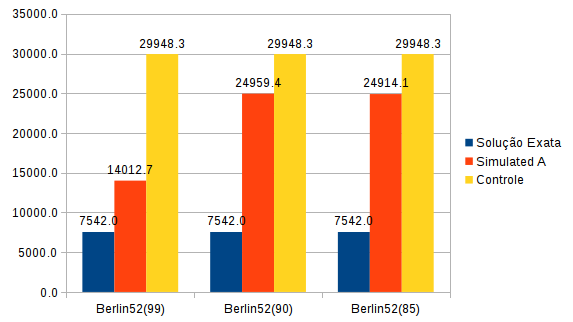
\includegraphics{figures/graph3.png}
	\caption{Gráfico comparativo de resultados - Berlin56.}
	\label{fig:graph1}
\end{figure}

\begin{figure}[H]
	\centering
	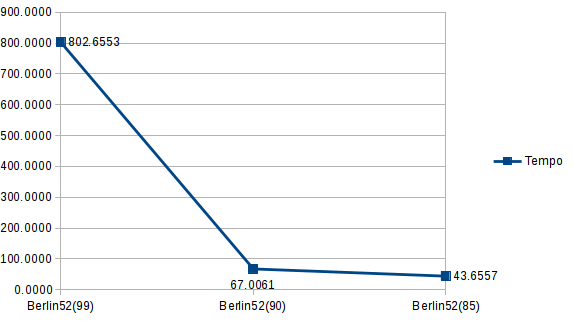
\includegraphics[scale=0.8]{figures/graph4.png}
	\caption{Gráfico comparativo de tempo - Berlin56.}
	\label{fig:graph2}
\end{figure}

\begin{figure}[H]%[!htbp]
	\centering
	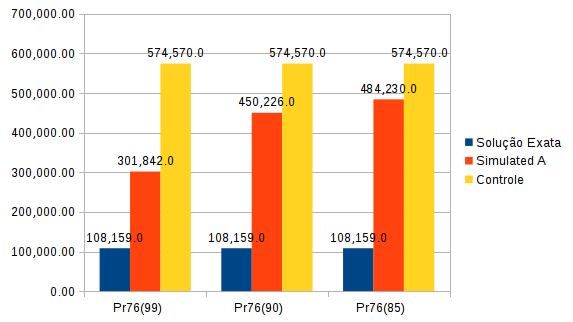
\includegraphics[scale=0.8]{figures/graph1.png}
	\caption{Gráfico comparativo de resultados - Pr76.}
	\label{fig:graph3}
\end{figure}

\begin{figure}[H]
	\centering
	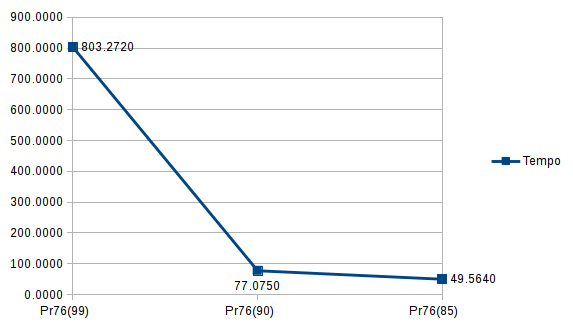
\includegraphics[scale=0.8]{figures/graph2.png}
	\caption{Gráfico comparativo de tempo - Pr76.}
	\label{fig:graph4}
\end{figure}

\begin{figure}[H]
	\centering
	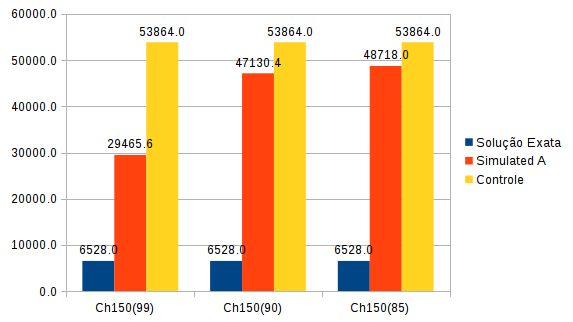
\includegraphics[scale=0.8]{figures/graph5.png}
	\caption{Gráfico comparativo de resultados - Ch150.}
	\label{fig:graph5}
\end{figure}

\begin{figure}[H]
	\centering
	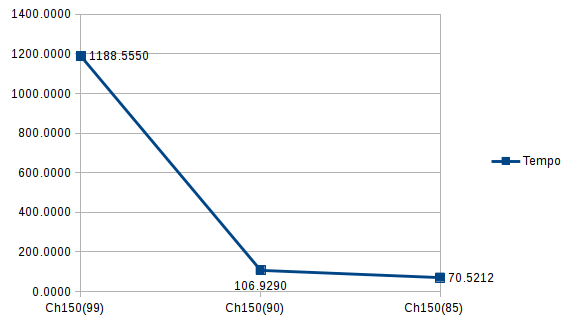
\includegraphics[scale=0.8]{figures/graph6.png}
	\caption{Gráfico comparativo de tempo - Ch150.}
	\label{fig:graph6}
\end{figure}

Conclui-se a partir dos dados analisados que a solução por \textit{simulated annealing}, em termos de qualidade de solução, sempre apresenta uma melhora em relação a valores aleatórios, porém piora significativa em relação à solução ótima. Por conta da manutenção dos dos parâmetros do \textit{simulated annealing} ao longo das execuções, instâncias menores apresentaram soluções de qualidade melhor que instâncias maiores.

A partir da análise dos dados referentes a execuções com alterações no parâmetro $\alpha$, percebe-se que para $\alpha = 0,99$, os tempos de execução são bastante elevados, ao passo que para os demais valores testados os tempos de execução são parecidos.

A qualidade das soluções encontradas acompanha, também, este padrão; portanto há soluções de qualidade razoavelmente melhor para $\alpha = 0,99$ em relação às demais soluções, as quais apresentam qualidade parecida. Observa-se, assim, a grande influência desse parâmetro no tempo de execução e qualidade das soluções.

\clearpage
\newpage
\subsection{Comparação com instâncias menores}

Como não foi possivel fazer os testes dos algoritimos exatos utilizando as entradas da literatura, foram feitos testes utilizando uma entrada menor. Na Tabela \ref{tab:bestLittle} apresentam-se as melhores soluções encontradas por nossos algoritmos exatos, a qual será utilizada como referência para a verificação da qualidade das soluções aproximadas, assim como a solução média gerada aleatoriamente:


\begin{table}[H]

\centering
\begin{tabular}{| l |  l |}
 \hline
 \textbf{Melhor valor encontrado} & 4564.46 \\
 \hline
\textbf{Melhor rota} & 1 6 2 7 8 9 10 12 11 3 5 4 0 1\\
 \hline
\textbf{Média das soluções aleatórias} & 11502.8\\
 \hline
\end{tabular}
\caption{\label{tab:bestLittle}Informações a respeito de soluções exatas para a instância \textit{littleboy}}
\end{table}

Soluções foram calculadas a partir da instância para os métodos aqui apresentados, o que permitiu verificar o tempo gasto pelos algoritmos. A Tabela \ref{tab:tempos} apresenta uma comparação entre os resultados obtidos, onde o parâmetro $\alpha$ da solução aproximada foi colocado como \textit{0,99}:

\begin{table}[H]

\centering
\begin{tabular}{| l | l | l | l | l | l |}
\hline
\textbf{Input} & \textbf{Abordagem }& \textbf{Solução} & \textbf{Random} & \textbf{Tempo(s)} \\\hline
littleboy & naive & 4564.46    & 11502.8 & 3349.47  \\\hline
littleboy & naive & 4564.46    & 11502.8 & 3360.01   \\\hline
littleboy & backtracking & 4564.46   & 11502.8  & 22.4283   \\\hline
littleboy & backtracking & 4564.46 & 11502.8     & 22.5526   \\\hline
littleboy & simulated annealing & 4660.45 & 11502.8     & 726.597    \\\hline
littleboy & simulated annealing & 4614.02 & 11502.8   & 726.275    \\\hline
\end{tabular}
\caption{\label{tab:tempos} Resultados obtidos para \textit{littleboy}}
\end{table}

A partir dos dados apresentados anteriormente é possível perceber que, para esta instância, a solução apresentada pelo \textit{simulated annealing} é bastante satisfatória; a partir de um valor médio dessas soluções, é possível perceber uma diferença de apenas 1,6\% em relação à solução exata, ao passo que a média de soluções aleatórias apresenta uma diferença de 
152\%. Seu tempo de execução, porém, se mostrou maior que o tempo de execução da solução por \textit{backtracking}, mas ainda razoavelmente menor que para a abordagem \textit{naive}.

	A fim de se verificar a melhora de tempo das abordagens \textit{backtracking} e \textit{simulated annealing}, calculou-se o \textit{speedup} da média destas em relação à abordagem \textit{naive}, onde $speedup = t_{naive}/t_{bt,sa}$. Os resultados obtidos apresentam-se na Tabela \ref{tab:spdup} e na Figura \ref{fig:speedup}:
    
 \begin{table}[H]
\centering
\begin{tabular}{| l | l | l | l | l}
\hline
\textbf{abordagem} & \textbf{tempo médio(s)} & \textbf{speedup} \\\hline
naive & 3354,74 & 1x \\\hline
backtracking & 22,49045 & 149x \\\hline
simulated annealing & 726,436 & 4,6x \\\hline
\end{tabular}
\caption{\label{tab:spdup} Dados a respeito do tempo de execução}
\end{table}

\begin{figure}[!htbp]
	\centering
	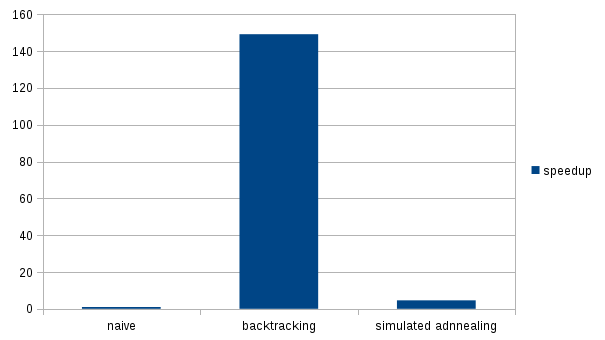
\includegraphics{figures/graph7.png}
	\caption{\label{fig:speedup}Gráfico comparativo de tempos de execução - \textit{littleboy}}
\end{figure}

Desta maneira, conclui-se que para instâncias de tamanho pequeno a solução por \textit{backtracking} é mais eficiente que a por \textit{simulated annealing}; conclui-se, também, que a solução aproximada apresenta qualidade muito boa e, portanto, mostra-se como uma boa alternativa à solução \textit{naive}.

Propõe-se, para trabalhos futuros, testes similares para o \textit{simulated annealing} com valores diferentes de $\alpha$, a fim de se verificar relações diferentes de custo-benefício quanto ao tempo de execução e a qualidade das soluções. A análise de tal valor, porém, estaria sujeita ao propósito das soluções em um problema do mundo real. 





%\textbf{Estimar tempo p/10}

%Res. ótimo: 2826.5

%Tempo: 0.064223

%\textbf{Estimar tempo da solução por backtraking baseado em parte da execução da Berlin52.}
%Para estimar o tempo de execução sa solução por backtracking para a entrada Berlin52, o algoritimo foi executado por 10 minutos, e durante a execução foi verificado o progresso atual, assim foi obtido...

\clearpage
\newpage


\section{Conclusão}

A partir dos testes realizados foi possível observar que as soluções exatas apresentam um tempo de execução bastante elevado, o que as torna impraticáveis para instâncias suficientemente grandes.

O método utilizado para soluções aproximadas apresentou resultados melhores do que a média de soluções aleatórias, mas distantes da solução ótima, especialmente em instâncias numerosas.

Para instâncias menores, porém, as soluções aproximadas apresentaram boa qualidade, mas uma vantagem menos expressiva em relação às soluções exatas.

Observou-se, também, resultados a partir da alteração de parâmetros dentro da solução aproximada.

Para um projeto futuro, seria interessante um refinamento mais criterioso da solução aproximada, de maneira que as soluções se aproximassem mais dos resultados conhecidos da literatura.


\newpage

\addcontentsline{toc}{section}{Bibliografia}
%\section*{Bibliografia}
\bibliography{bibliography}
\bibliographystyle{plain}
\newpage
\addcontentsline{toc}{section}{Anexo}
%\section*{Anexo}
\end{document}



